\documentclass[12pt, spanish]{article}
\usepackage[spanish]{babel}
\selectlanguage{spanish}
\usepackage[utf8]{inputenc}
\usepackage{amsmath}
\usepackage{newfloat}
%\usepackage{fullpage}
\usepackage[top=0.80in, bottom=0.80in, left=0.85in, right=0.85in]{geometry}
\usepackage{multicol}
\usepackage{wrapfig}
\usepackage{enumerate}
\usepackage{graphicx}
\usepackage{newfloat}
\usepackage{geometry}
\usepackage{array}
\usepackage{hyperref}
\usepackage{multirow}
\usepackage{multicol}
\usepackage{float}
\restylefloat{table}
\renewcommand{\baselinestretch}{1.5}
\begin{document}
\title{Tarea 1 - Semana 4}


\thispagestyle{empty}
\begin{center}

\includegraphics[width=12cm]{Universidad_San_Andres_UdeSA.jpg}
\end{center}

	\begin{center}
	\LARGE
\textbf{HERRAMIENTAS COMPUTACIONALES PARA INVESTIGACIÓN}
	

	\vspace{1.5 cm}
	\LARGE
	\textit{Tarea 1 - Semana 4}

	\vspace{1 cm}
	\Large
	Clara Pasman \& Rosario Podestá\
	
	\vspace{1.3cm}
	\Large	
	Profesora: Amelia Gibbons\

	
	\vspace{1 cm}
	\normalsize
	\today
	\end{center}
	
\clearpage

\begin{figure}
    \centering
    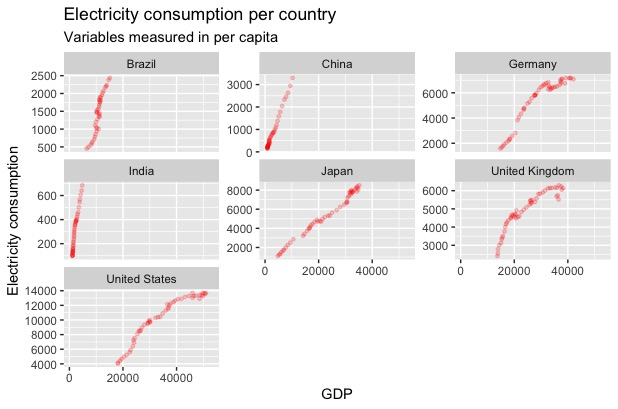
\includegraphics[width=15cm]{Electricity Consumption.jpeg}
    \caption{}
    \label{fig:my_label}
\end{figure}
Para este gráfico mantuvimos el formato origianl y añadimos color en degradé para las observaciones, dejamos variar el eje y para cada país, y agregamos etiquetas y títulos. 

\clearpage

\begin{figure}
    \centering
    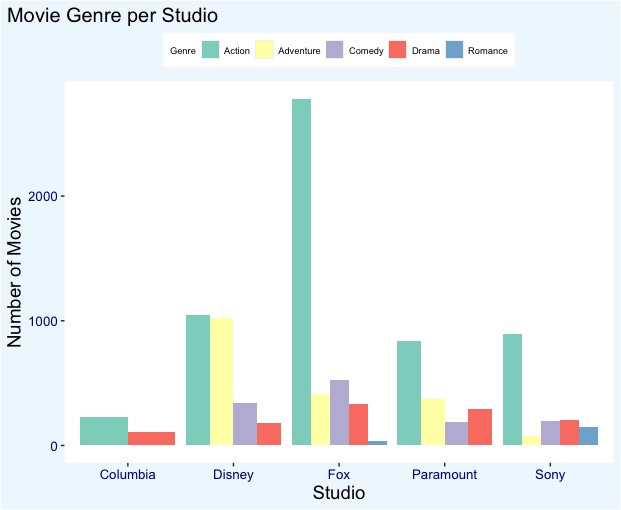
\includegraphics[width=15cm]{Movie Genre.jpeg}
    \caption{}
    \label{fig:my_label}
\end{figure}

En este caso, cambiamos la variable x. Creemos que la cantidad de películas de cada estudio para los distintos géneros se visualizaba mejor de la forma presentada. Además de cambiar el \textit{theme} del histgrama, agregamos un título y modificamos las etiquetas. 
\clearpage

\begin{figure}
    \centering
    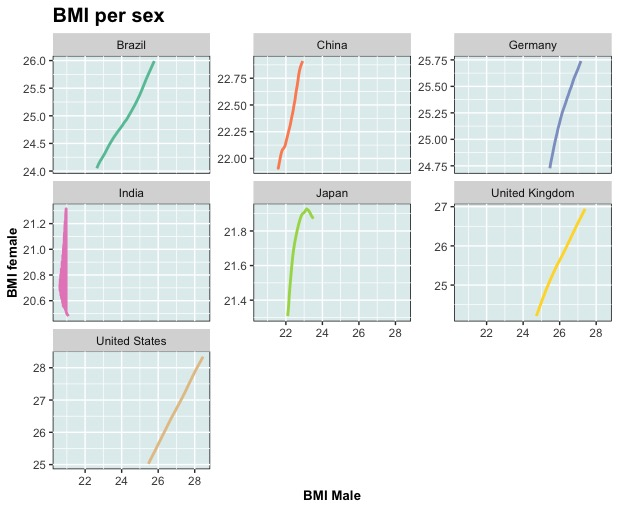
\includegraphics[width=15cm]{BMI.jpeg}
    \caption{}
    \label{fig:my_label}
\end{figure}
Separamos en gráficos individuales la relación entre el índice de masa corporal de hombres y mujeres para cada país. También  modificamos el \textit{theme} y dejamos variar el eje y para cada país en particular. 



\end{document}
